\documentclass[paper=a4, fontsize=12pt]{scrartcl} % A4 paper and 11pt font size
\usepackage[margin=1in]{geometry}  

\usepackage[T1]{fontenc} % Use 8-bit encoding that has 256 glyphs
\usepackage{fourier} % Use the Adobe Utopia font for the document - comment this line to return to the LaTeX default
\usepackage[english]{babel} % English language/hyphenation
\usepackage{amsmath,amsfonts,amsthm} % Math packages
\usepackage{enumerate}
\usepackage{graphicx}
\usepackage{caption}

\usepackage{sectsty} % Allows customizing section commands
\allsectionsfont{\raggedright \normalfont\scshape} % Make all sections centered, the default font and small caps

\usepackage{fancyhdr} % Custom headers and footers
\pagestyle{fancyplain} % Makes all pages in the document conform to the custom headers and footers
\fancyhead[R]{\emph{Flow Past Objects - Chapter 4}} % No page header - if you want one, create it in the same way as the footers below
\fancyfoot[L]{} % Empty left footer
\fancyfoot[C]{} % Empty center footer
\fancyfoot[R]{\thepage} % Page numbering for right footer
\renewcommand{\headrulewidth}{0pt} % Remove header underlines
\renewcommand{\footrulewidth}{0pt} % Remove footer underlines
\setlength{\headheight}{13.6pt} % Customize the height of the header

\numberwithin{equation}{section} % Number equations within sections (i.e. 1.1, 1.2, 2.1, 2.2 instead of 1, 2, 3, 4)
\numberwithin{figure}{section} % Number figures within sections (i.e. 1.1, 1.2, 2.1, 2.2 instead of 1, 2, 3, 4)
\numberwithin{table}{section} % Number tables within sections (i.e. 1.1, 1.2, 2.1, 2.2 instead of 1, 2, 3, 4)

%----------------------------------------------------------------------------------------
%	TITLE SECTION
%----------------------------------------------------------------------------------------

\newcommand{\horrule}[1]{\rule{\linewidth}{#1}} % Create horizontal rule command with 1 argument of height

\author{\vspace{-5ex}}
\date{\vspace{-10ex}}
\title{	
\normalfont \normalsize 
\textsc{Chem-Eng 321: Fluid Mechanics} \\ [10pt] % Your university, school and/or department name(s)
\horrule{0.5pt} \\[0.2cm] % Thin top horizontal rule
\huge Flow Past Objects \\ (Denn Chapter 4) \\ % The assignment title
\horrule{2pt} \\[0.2cm] % Thick bottom horizontal rule
}


\begin{document}

\maketitle % Print the title

\thispagestyle{empty}

\section*{Learning Objectives}

\begin{enumerate}
\item Relate and calculate the Drag Coefficient ($c_D$) to fluid and object parameters for different Reynold's number regions.
\item Derive and apply terminal (settling) velocity as a function of fluid and object parameters.
\item Derive and apply a model for fluid flow through packed bed systems.
\end{enumerate}

\section*{Introduction}

Why do engineers care about flow past an object?


\vspace{10ex} \section*{Flow past a sphere}
Consider flow past a sphere:


\begin{figure}[ht]
\centering
\begin{minipage}[b]{0.45\linewidth}
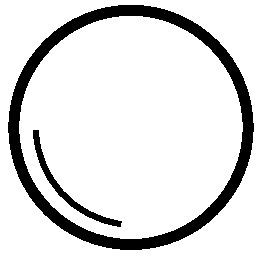
\includegraphics[scale=0.8]{sphere.pdf}
\end{minipage}
\quad
\begin{minipage}[b]{0.45\linewidth}
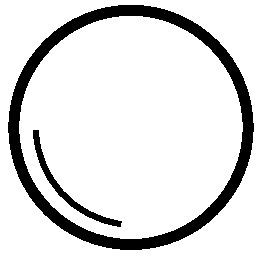
\includegraphics[scale=0.8]{sphere.pdf}
\end{minipage}
\end{figure}

How does drag force $F_D$ depend on...


\subsection*{Dimensional Analysis}
\begin{tabular}{ c || l  }
  Variable & Dimensions (Length, Time, Mass) \\
  $F_D$  & $\frac{ML}{T^2}$  \\
   &   \\
   &   \\
   &   \\
   &   \\
   &   \\
   &   \\
   &   \\
   &   \\
   &   \\
   &   \\
   &   \\
   &   \\
\end{tabular}


Many options; conventions dictate:

\vspace{5ex} \begin{equation*}
\hspace*{-7cm}  \text{Re}= \hspace*{7cm}  c_D=
\end{equation*}

\vspace{5ex}  For the drag coefficient $c_D$, the general definition is

\vspace{4cm} \begin{equation*}
\hspace*{-7cm}  c_D=f(\text{Re})
\end{equation*}
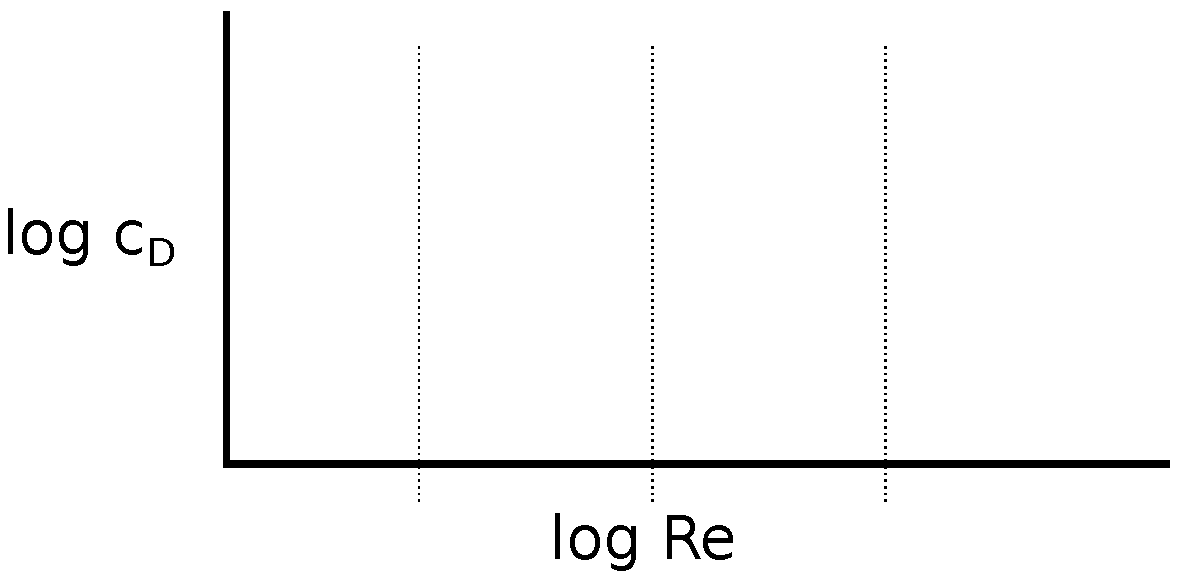
\includegraphics[scale=0.6]{cdvsre.pdf}

\newpage


\section*{Representation of Data}

\subsection*{Small Re (<1)}
Find that $c_D \propto \frac{1}{\text{Re}}$. In fact, $c_D=$



\vspace{4cm} \subsection*{Intermediate Region (1<Re<$10^3$)}
\vspace{4ex} \begin{equation*}
\hspace*{-7cm} c_D=
\end{equation*}

\vspace{4ex} \subsection*{Large Re ($10^3$<Re<$2 \times 10^5$)}
\vspace{4ex} \begin{equation*}
\hspace*{-7cm} c_D \approx
\end{equation*}

\vspace{4ex}  For Re = $2 \times 10^5$, sharp drop...

\newpage

\section*{Terminal Velocity}
Sphere falling/rising in fluid by gravitational force.

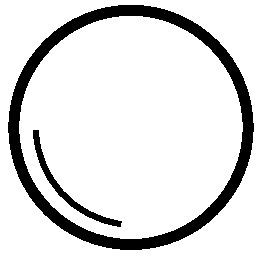
\includegraphics[scale=0.6]{sphere.pdf}

\vspace{6cm} Stokes regime: 

\vspace{2cm}  Newton regime:

\newpage
\section*{Other Shapes}
\hspace*{1cm}  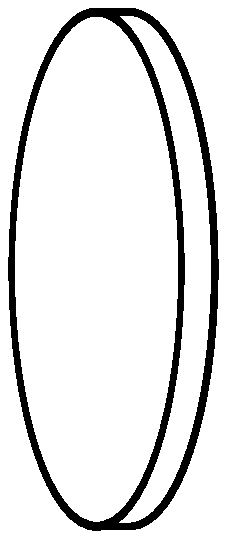
\includegraphics[scale=0.5]{circulardisk.pdf}

\vspace{0.5cm}  \hspace*{0.5cm}  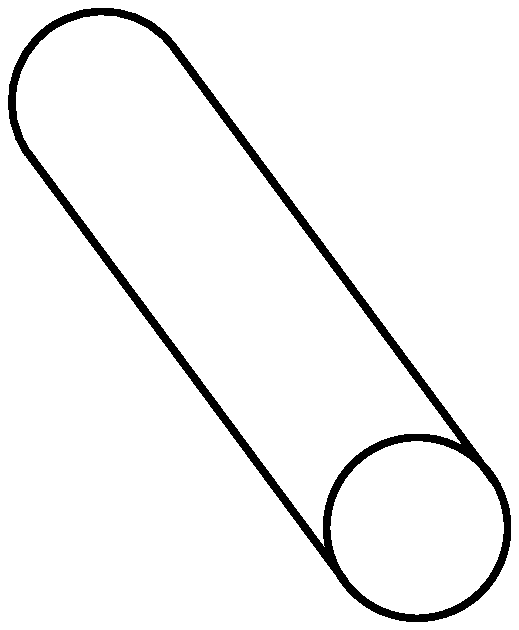
\includegraphics[scale=0.3]{cylinder.pdf}

\vspace{2cm}   \section*{Handouts}

Table 9.4 from Munson, Young, and Okiishi. Fundamentals of Fluid Mechanics, 5th edition.

Comments
\begin{itemize}
  \item ~
  \vspace{1.5cm}  \item 
  \item  
\end{itemize}

Flow Patterns/Discussion $\rightarrow$ DVD-ROM

\begin{itemize}
  \item 
  \item ~
  \vspace{.5cm}  \item  
  \item
\end{itemize}

\newpage

\section*{Example}
How much energy does the 1992 version of Professor Burghardt expend to overcome aerodynamic drag while running a complete marathon race on a day with no wind? Assume that he completed a marathon in 3 hours.

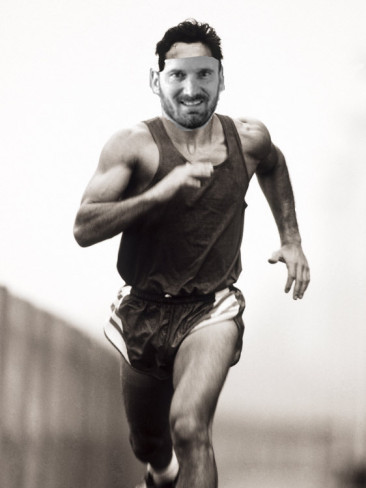
\includegraphics[scale=0.5]{wesrunning.jpg}

\vspace{11cm}  Now suppose that Professor Burghardt had used that energy instead to power a light bulb (100 watts). How long could he generate light for a family in India who doesn't have access to electricity?

\newpage

\section*{Packed Beds}
\vspace{0.5cm}  \hspace*{0.5cm}  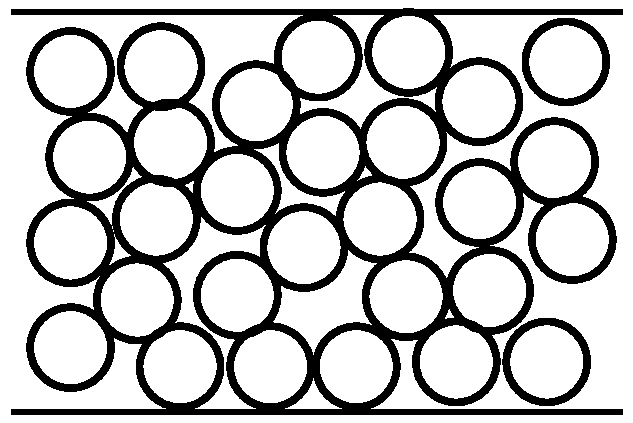
\includegraphics[scale=0.6]{packedbed.pdf}




\vspace{0.5cm}   Uses:
\begin{itemize}
  \item 
  \item 
  \item  
\end{itemize}

"Void Fraction" = $\varepsilon$ =

\vspace{0.8cm}   "Superficial velocity" = $v_{\infty}$ =

\vspace{0.5cm}   How does $\Delta p$ depend on...


\vspace{1cm}   Approach: Think of fluid's path through  packing as a complicated "pipe"

\vspace{0.5cm}   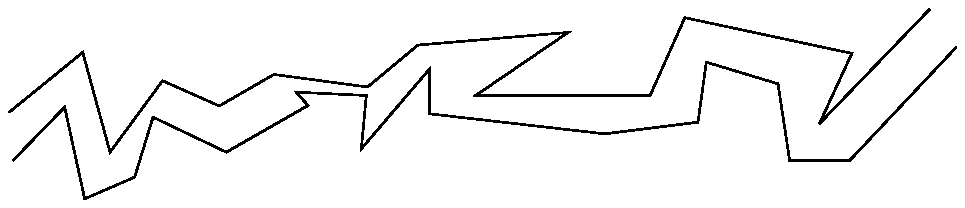
\includegraphics[scale=0.8]{crazypipe.pdf}

For pipe flow, correlate data: 

\newpage
 Problem: How do $D_{\text{eff}}$ and $v_{\text{eff}}$ relate to measurable variables?

\begin{enumerate}
  \item 

 \item \vspace{2cm}  Set $D_{\text{eff}}=D_H$ (hydraulic diameter) \\
 
 
\vspace{1.5cm}  $V_{\text{fluid}}$ - Volume of the fluid \hspace{0.5cm}  $V_{\text{solids}}$ - Volume of the solid particles

 $V_{\text{bed}}$ - Volume of the bed ($V_{\text{bed}}=V_{\text{fluid}}+V_{\text{solids}}$)

\vspace{4cm} Let $N_p$ be the number of particles in the bed



\vspace{8cm}  $D_{\text{eff}}=$

\end{enumerate}

\newpage

\vspace{0.5cm} Plug back into the correlation: 

\vspace{1.5cm} Normally drop numerical factors, and represent data according to:
\vspace{4ex} \begin{equation*}
\hspace*{-7cm} \text{f}_{\text{p}}=f_{\text{p}}(\text{Re}_{\text{p}})
\end{equation*}

\vspace{3cm} Experimental Data

 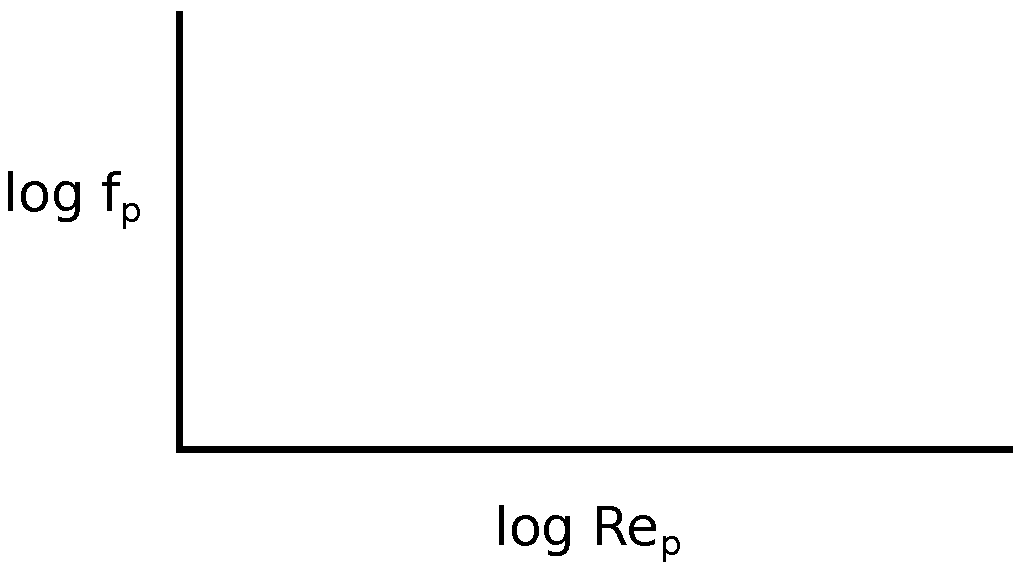
\includegraphics[scale=0.6]{fpvsrep.pdf}
 
\vspace{0.5cm} Data correlation. Ergun Equation:  $f_{\text{p}}=$

\vspace{0.5cm} For low Re$_\text{p}$, we can neglect the constant term

\newpage

\section*{Fluidized beds}

 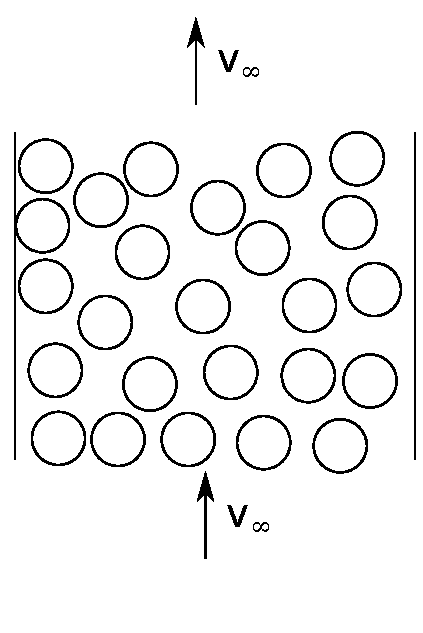
\includegraphics[scale=0.6]{packedbedvert.pdf}



\vspace{1cm}  \section*{Chapter Summary}

In this chapter we consider flow past objects in technically relevant areas for engineers
	
\begin{itemize}
  \item 
  \item 
  \item
\end{itemize}

We developed a model to relate drag force $F_D$ to fluid and object parameters. In particular, we use the dimensionless group $c_D$ against Reynold's number (Re).

\newpage

 \section*{Appendix A}

 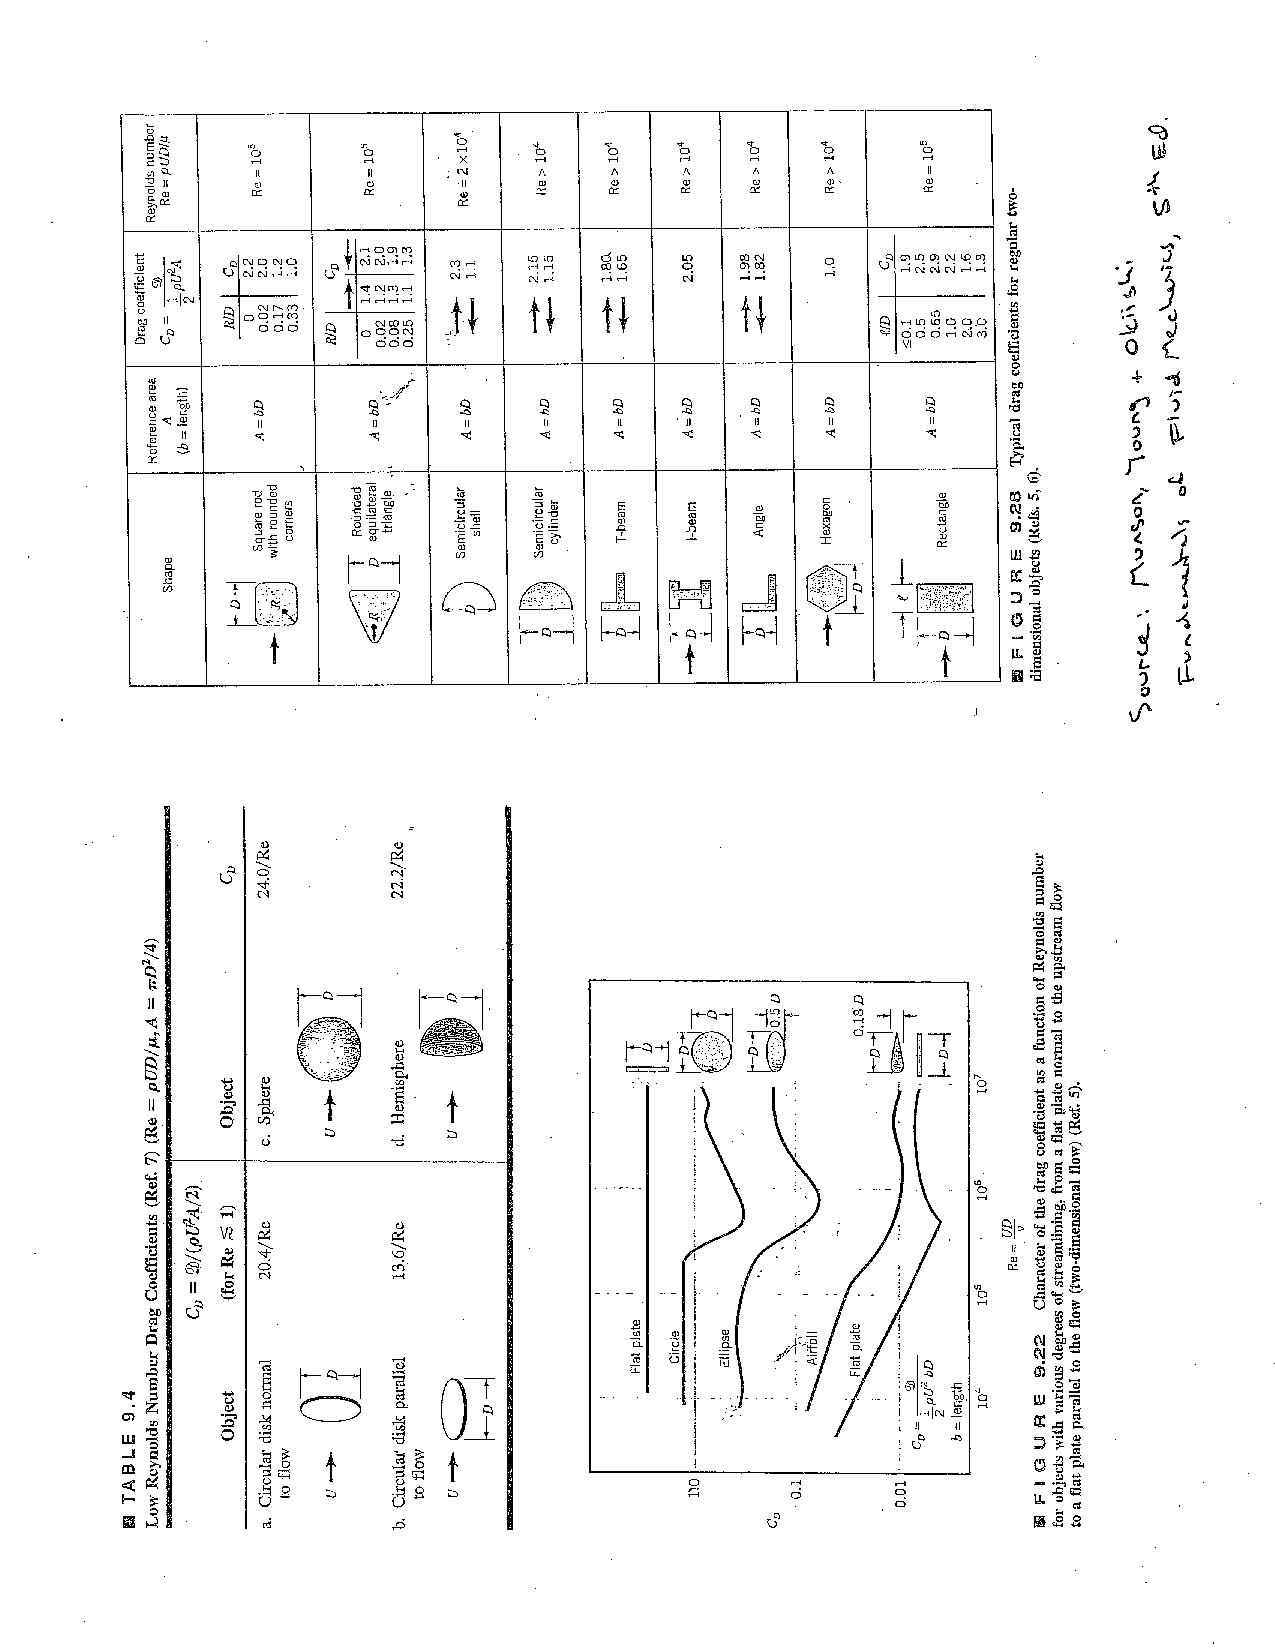
\includegraphics[scale=0.90]{Munsonfigure94.pdf}
 
 \newpage
 
  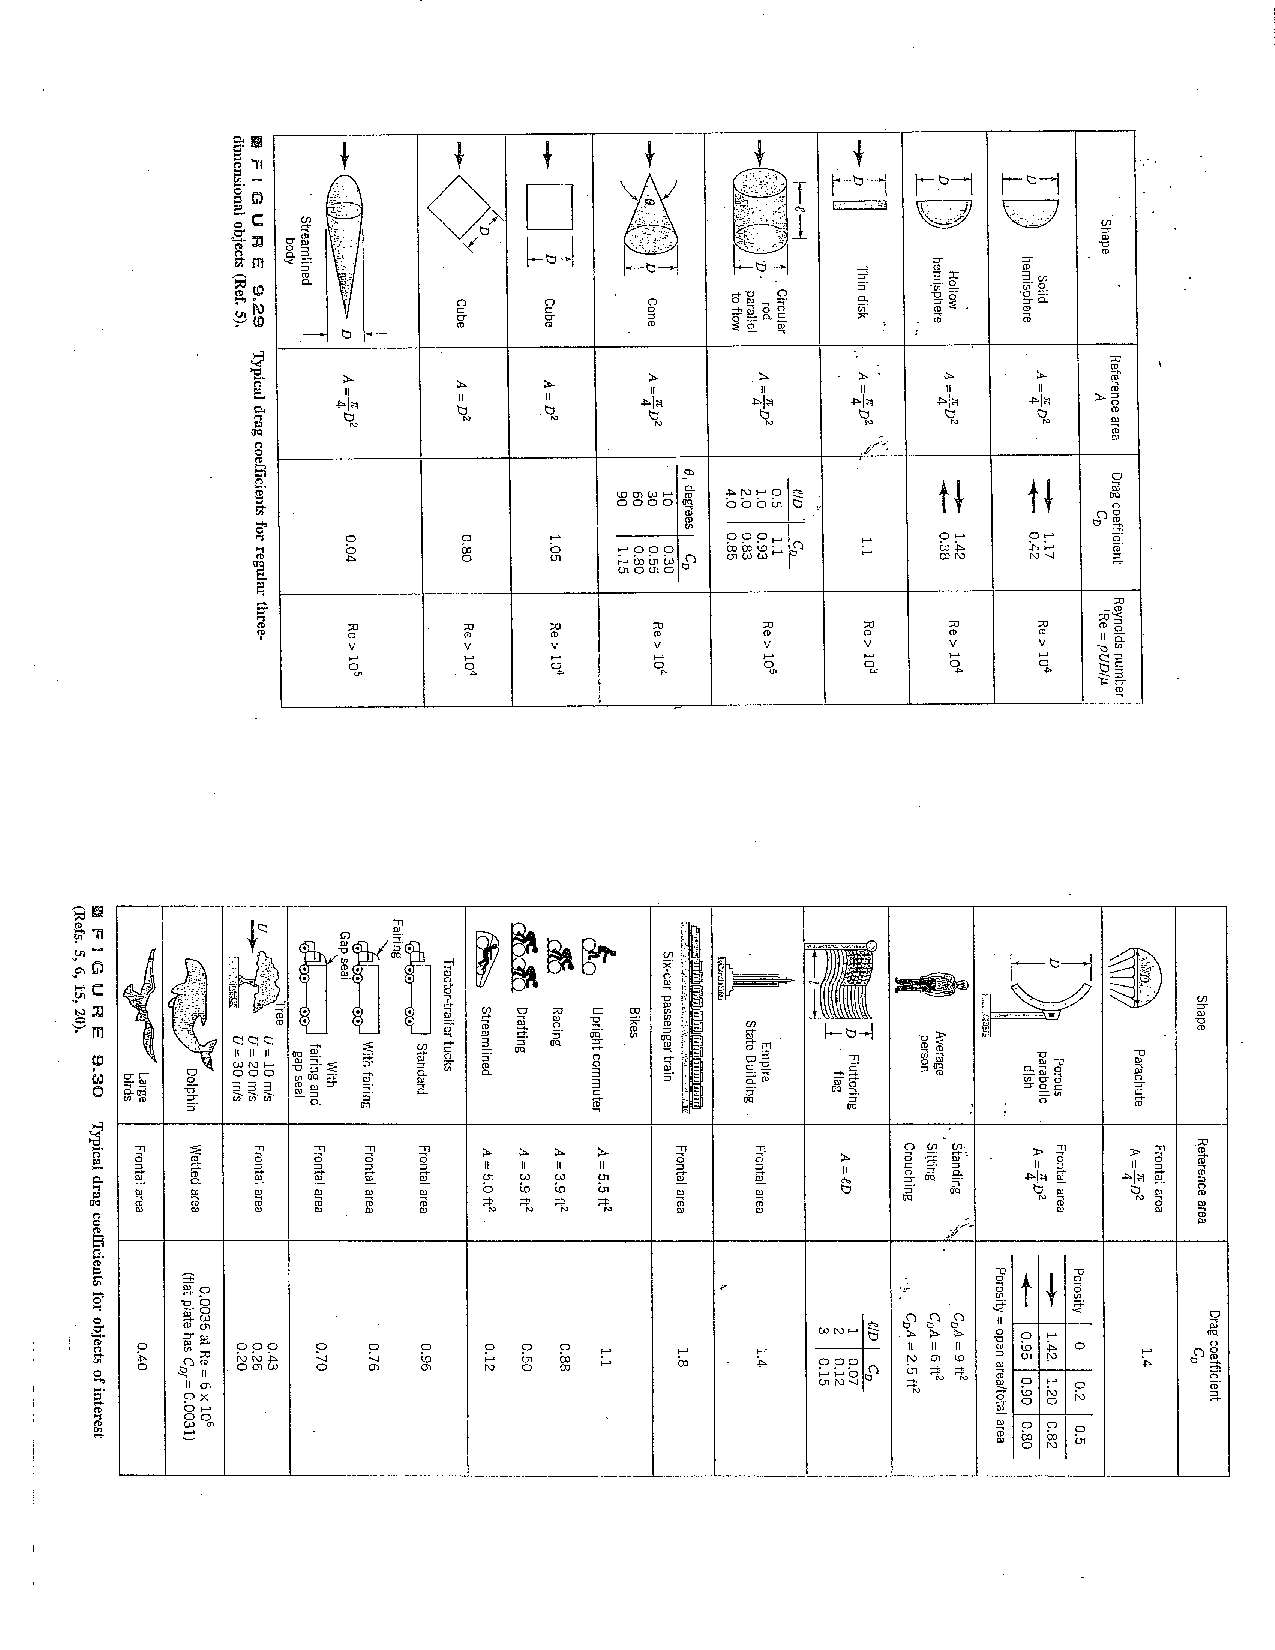
\includegraphics[scale=0.80]{Munsonfigure94Part2.pdf}
  
   \newpage

 \section*{Packed Bed Example}

Suppose cylindrically shaped particles with diameters of 0.5 mm and lengths of 1 mm are packed into a space with a diameter of 50 mm and length of 15 mm. The mass flow rate is $4 \times 10^{-4}$ kg/s. The liquid density and viscosity are 1200 kg/m$^3$ and 700 Pa s respectively. What's the pressure drop if the void fraction $\varepsilon$ is 0.4?
\end{document}